\documentclass[12pt, aspectratio=169]{beamer}

\usetheme{Madrid}
\usecolortheme{whale}
\setbeamertemplate{navigation symbols}{}
\setbeamertemplate{footline}[frame number]

\usepackage{amsmath, amssymb}
\usepackage{booktabs}
\usepackage{array}
\usepackage{xcolor}
\usepackage{tikz}
\usepackage{pgfplots}
\pgfplotsset{compat=1.18}
\usetikzlibrary{arrows.meta, positioning}

\definecolor{whartonblue}{RGB}{0,51,102}
\definecolor{whartonorange}{RGB}{204,102,0}
\definecolor{whartonred}{RGB}{153,0,0}

\setbeamercolor{structure}{fg=whartonblue}
\setbeamercolor{frametitle}{bg=whartonblue, fg=white}
\setbeamercolor{title}{fg=white}
\setbeamercolor{subtitle}{fg=white}
\setbeamercolor{author}{fg=white}
\setbeamercolor{date}{fg=white}
\setbeamercolor{institute}{fg=white}

\title{Valuing and Pricing Financial Datasets}
\subtitle{From Predictive Power to Economic Value}
\author{Bailey McIntosh}
\institute{Wharton Research Scholars}
\date{April 2026}

\begin{document}

% -------------------------------------------------------
\begin{frame}
  \titlepage
\end{frame}

% -------------------------------------------------------
\begin{frame}{Research Question}

\textbf{How should a financial dataset be priced?}

\medskip
\begin{itemize}\setlength\itemsep{6pt}
  \item Data is the input that forms investor beliefs; beliefs determine
        portfolios; portfolios aggregate into order flow; order flow determines
        prices. \emph{The distribution of data access directly determines how
        efficiently prices aggregate information across the economy.}
  \item As quantitative methods diffuse broadly, the scarce factor shifts from
        modeling skill to proprietary data --- whoever controls the signal
        controls the edge.
  \item Yet data markets are almost entirely \textbf{private and opaque}:
        no observable prices, no standard contracts, no theory of how they work.
\end{itemize}

\medskip
\textbf{Two questions this paper addresses:}
\begin{enumerate}
  \item What is a dataset worth to a single investor?
  \item How does a data vendor optimally price and license that dataset?
\end{enumerate}

\end{frame}

% -------------------------------------------------------
\begin{frame}{Value = PV of Incremental Trading Profits}

\begin{columns}[T]
\begin{column}{0.53\textwidth}
\footnotesize
\textbf{Pay for data what the extra profits it generates are worth,
discounted over your investment horizon:}
\vspace{2pt}
\[
  V_i(D) \;=\; \sum_{t=1}^{T}
    \frac{\mathbb{E}[\Delta CF_{i,t}(D)]}{(1+r_i)^{t}}
    \;-\; C_i(D)
\]
\vspace{-4pt}
$\Delta CF_{i,t}$ = incremental trading profit from $D$ in period $t$;
$C_i(D)$ = acquisition cost.

\smallskip
\textbf{$\Delta CF_{i,t}$ is the product of two objects:}
\begin{itemize}\setlength\itemsep{1pt}
  \item the \emph{predictive edge} $D$ adds over existing information ($\Delta R^2$)
  \item the \emph{capital profitably deployable} on that edge
\end{itemize}

\smallskip
Both are endogenous to market structure. Three dynamics determine them.
\end{column}

\begin{column}{0.44\textwidth}
\vspace{0.2cm}
\centering
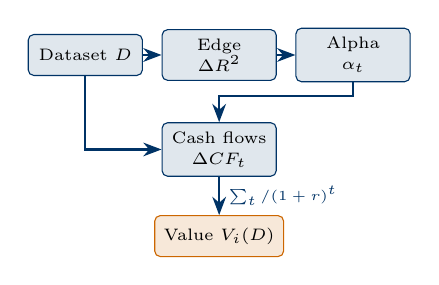
\begin{tikzpicture}[
  box/.style={rectangle, rounded corners=2pt, draw=whartonblue,
              fill=whartonblue!12, align=center,
              font=\fontsize{6.5}{7.5}\selectfont,
              minimum width=1.45cm, minimum height=0.52cm},
  obox/.style={rectangle, rounded corners=2pt,
               draw=whartonorange, fill=whartonorange!15,
               align=center, font=\fontsize{6.5}{7.5}\selectfont,
               minimum width=1.45cm, minimum height=0.52cm},
  arr/.style={-Stealth, thick, color=whartonblue}
]
\node[box] (D)  at (0,0)   {Dataset $D$};
\node[box] (R)  at (1.7,0) {Edge\\$\Delta R^2$};
\node[box] (A)  at (3.4,0) {Alpha\\$\alpha_t$};
\node[box] (CF) at (1.7,-1.2) {Cash flows\\$\Delta CF_t$};
\node[obox](V)  at (1.7,-2.3) {Value $V_i(D)$};
\draw[arr] (D)  -- (R);
\draw[arr] (R)  -- (A);
\draw[arr] (A)  -- ++(0,-0.52) -| (CF);
\draw[arr] (D)  -- ++(0,-1.2) -- (CF);
\draw[arr] (CF) -- node[right, font=\fontsize{5.5}{6.5}\selectfont]
                   {$\sum_t/(1+r)^t$} (V);
\end{tikzpicture}
\vspace{0.15cm}

{\fontsize{7}{8.5}\selectfont\itshape
Value is investor-specific ($\bar{w}_i$, $\gamma_i$, style),
forward-looking, and endogenous to market structure.}
\end{column}
\end{columns}

\end{frame}

% -------------------------------------------------------
\begin{frame}{Three Dynamics That Complicate Valuation}

\small\textbf{Each component of $\Delta CF_{i,t}(D)$ is endogenous:}

\smallskip
\begin{columns}[T]

\begin{column}{0.31\textwidth}
\begin{block}{\centering\small 1.\; Market Size}
\footnotesize\smallskip
Even with unlimited capital, cash flows from a signal are \textbf{bounded
by market depth}. A signal on a small or illiquid universe hits a hard
ceiling on extractable profit regardless of predictive accuracy.
\end{block}
\end{column}

\begin{column}{0.31\textwidth}
\begin{block}{\centering\small 2.\; Deployable Capital}
\footnotesize\smallskip
Value scales with AUM \textbf{up to the point where position size exceeds
market absorption capacity}. Beyond that, price impact erases gains.
The AUM--value relationship is concave, not linear.
\end{block}
\end{column}

\begin{column}{0.31\textwidth}
\begin{block}{\centering\small 3.\; Adoption}
\footnotesize\smallskip
As $n$ investors trade the same signal, they \textbf{collectively reveal it
to the market}. Cash flows shrink for all holders as the mispricing is
corrected faster. Value is endogenous to who else owns the data.
\end{block}
\end{column}

\end{columns}

\medskip
{\small
Together these dynamics explain why \emph{statistical accuracy is neither
necessary nor sufficient for economic value} --- the central puzzle this
paper resolves.}

\end{frame}

% -------------------------------------------------------
\begin{frame}{Contribution}

\small
Farboodi, Singal, Veldkamp, and Venkateswaran (2021) derive the private value
of a dataset to a single investor and explicitly set aside two next steps.
This paper takes both, plus a third.

\smallskip
\begin{enumerate}\setlength\itemsep{7pt}
  \item \textbf{Prediction-to-precision bridge.}
        Maps observable metrics ($\Delta R^2$, MSE) to the signal precision
        parameters that enter the valuation formula --- making the cash-flow
        framework computable from numbers practitioners actually report.

  \item \textbf{Equilibrium transaction prices.}
        Derives the vendor's optimal licensing problem: how many licenses to
        sell and at what price. Private value $\neq$ transaction price.

  \item \textbf{Competitive adoption as a first-order mechanism.}
        As $n$ investors share and trade the same signal, crowding erodes
        $\Delta CF_{i,t}$ for all holders. Introduces \emph{dataset capacity}
        $C(D)$ --- the rate at which this erosion occurs --- as a formal object.
\end{enumerate}

\end{frame}

% -------------------------------------------------------
\begin{frame}{Literature}

\textbf{Five strands --- one gap}

\vspace{2pt}
{\footnotesize
\renewcommand{\arraystretch}{1.05}
\begin{tabular}{@{} p{2.6cm} p{5.4cm} p{4.0cm} @{}}
\toprule
\textbf{Strand} & \textbf{Key insight} & \textbf{Role here} \\
\midrule
Costly information
  & Grossman-Stiglitz (1980): informed investors must earn rents or no one gets informed
  & Why datasets have value at all \\
Data valuation
  & Farboodi et al.\ (2021): private value via sufficient statistics
  & Direct foundation; extended here \\
Info.\ monopoly
  & Admati-Pfleiderer (1986): seller faces price vs.\ adoption tradeoff
  & Vendor pricing framework \\
Crowding \& decay
  & Kyle (1985); Holden-Subrahmanyam (1992); McLean-Pontiff (2016)
  & Micro-foundation for erosion \\
Club goods
  & Buchanan (1965): optimal club size under congestion
  & Structure of the $n^*$ problem \\
\bottomrule
\end{tabular}
}

\vspace{1pt}
\textbf{The gap:} No existing paper derives a transaction price for data
accounting for both investor heterogeneity and endogenous value erosion.

\end{frame}

% -------------------------------------------------------
\begin{frame}{Model}

\footnotesize

\textbf{Setup:} $N$ risky assets; CARA investors heterogeneous in AUM
$\bar{w}_i$, risk aversion $\gamma_i$, and style $\mathcal{Q}_i$.
Dataset $D$ produces a Gaussian signal about dividend innovations.
Noisy rational expectations equilibrium.

\smallskip
\textbf{Three components:}

\begin{enumerate}\setlength\itemsep{2pt}

  \item \textbf{Prediction-precision bridge} --- connects observable $\Delta R^2$
  to signal precision $K_i(D)$:
  \vspace{-4pt}
  \[
    K_i(D) = \frac{\Delta R^2(D)\cdot\sigma^2_y}
                  {\mathrm{MSE}_D\cdot\bigl(1-\Delta R^2(D)\bigr)}
  \]
  \vspace{-10pt}

  \item \textbf{Private value} (closed form, proportional to AUM, convex in $\Delta R^2$):
  \vspace{-4pt}
  \[
    V_i(D) \approx
    \frac{\bar{w}_i}{2\gamma_i}
    \cdot\frac{\Delta R^2(D)}{1-\Delta R^2(D)}
    \cdot\frac{\sigma^2_y}{\mathrm{MSE}_D}
    - C_i(D)
  \]
  \vspace{-10pt}

  \item \textbf{Crowding} --- $n$ investors sharing the signal trade more
  aggressively (Holden-Subrahmanyam 1992), raising Kyle $\lambda(n)$ and
  reducing each investor's profit. $C(D)$ parametrizes how fast aggregate
  informed order flow becomes detectable in the market.

\end{enumerate}

\end{frame}

% -------------------------------------------------------
\begin{frame}{Key Results}

\footnotesize

\begin{block}{Proposition 1 \;---\; Optimal Licensing}
Vendor maximizes revenue at $n^* = (C(D)+1)/2$ licenses.
Low-capacity datasets should be licensed exclusively;
high-capacity datasets sustain broad licensing.
\end{block}

\begin{block}{Proposition 2 \;---\; First-Mover Value Premium}
The $k$-th adopter captures more value than the $(k+1)$-th.
Premium is largest at the exclusive-to-shared transition and declines
monotonically. Early movers capture peak alpha; late movers may find
the data worthless.
\end{block}

\begin{block}{Proposition 3 \;---\; Information Seller's Paradox}
High accuracy ($\Delta R^2 \approx 1$) can coexist with zero or negative
economic value when capacity is low and adoption is broad.
\end{block}

\vspace{1pt}
\textbf{Further:} Large investors are more crowding-sensitive (Prop.\ 4);
revenue is monotone in quality \emph{and} capacity (Prop.\ 6).

\end{frame}

% -------------------------------------------------------
\begin{frame}{Visual Intuition}

\begin{columns}[T]

\begin{column}{0.48\textwidth}
\centering
{\small\textbf{Inverted Network Effect}}\\[1pt]
{\fontsize{7}{8}\selectfont Per-investor value as adoption grows (Props.\ 2 \& 3)}\\[3pt]
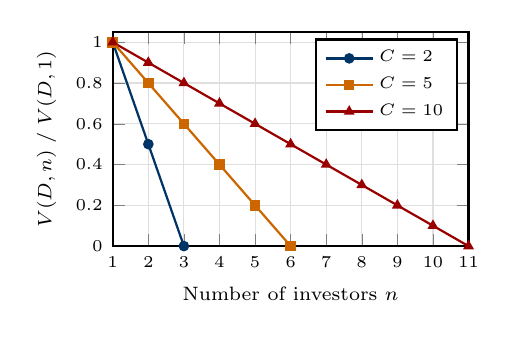
\begin{tikzpicture}
\begin{axis}[
  width=6.1cm, height=4.3cm,
  xlabel={\fontsize{7}{8}\selectfont Number of investors $n$},
  ylabel={\fontsize{7}{8}\selectfont $V(D,n)\;/\;V(D,1)$},
  xmin=1, xmax=11, ymin=0, ymax=1.05,
  xtick={1,2,...,11}, ytick={0,0.2,0.4,0.6,0.8,1.0},
  tick label style={font=\fontsize{6}{7}\selectfont},
  label style={font=\fontsize{7}{8}\selectfont},
  legend style={font=\fontsize{6}{7}\selectfont,
                at={(0.97,0.97)}, anchor=north east,
                cells={anchor=west}},
  grid=major, grid style={gray!25}, thick
]
\addplot[color=whartonblue, mark=*, mark size=1.5pt]
  coordinates {(1,1)(2,0.5)(3,0)};
\addlegendentry{$C=2$}
\addplot[color=whartonorange, mark=square*, mark size=1.5pt]
  coordinates {(1,1)(2,.8)(3,.6)(4,.4)(5,.2)(6,0)};
\addlegendentry{$C=5$}
\addplot[color=whartonred, mark=triangle*, mark size=1.5pt]
  coordinates {(1,1)(2,.9)(3,.8)(4,.7)(5,.6)(6,.5)(7,.4)(8,.3)(9,.2)(10,.1)(11,0)};
\addlegendentry{$C=10$}
\end{axis}
\end{tikzpicture}
\end{column}

\begin{column}{0.48\textwidth}
\centering
{\small\textbf{Vendor's Optimal Licensing}}\\[1pt]
{\fontsize{7}{8}\selectfont Revenue $R(n)=n\cdot V(D,n)$, normalized; $C=5$}\\[3pt]
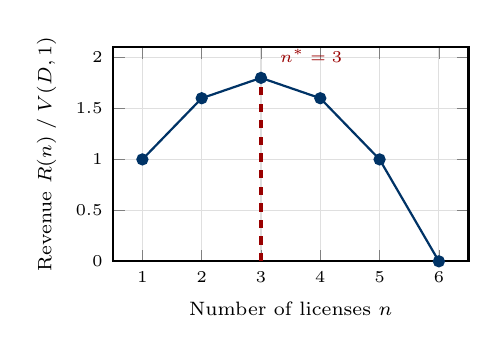
\begin{tikzpicture}
\begin{axis}[
  width=6.1cm, height=4.3cm,
  xlabel={\fontsize{7}{8}\selectfont Number of licenses $n$},
  ylabel={\fontsize{7}{8}\selectfont Revenue $R(n)\;/\;V(D,1)$},
  xmin=0.5, xmax=6.5, ymin=0, ymax=2.1,
  xtick={1,2,3,4,5,6}, ytick={0,0.5,1.0,1.5,2.0},
  tick label style={font=\fontsize{6}{7}\selectfont},
  label style={font=\fontsize{7}{8}\selectfont},
  grid=major, grid style={gray!25}, thick
]
\addplot[color=whartonblue, mark=*, mark size=1.8pt]
  coordinates {(1,1)(2,1.6)(3,1.8)(4,1.6)(5,1.0)(6,0)};
\addplot[dashed, color=whartonred, very thick]
  coordinates {(3,0)(3,1.8)};
\node at (axis cs:3.15,1.85)
  [font=\fontsize{6.5}{7.5}\selectfont, color=whartonred, anchor=south west]
  {$n^*=3$};
\end{axis}
\end{tikzpicture}
\end{column}

\end{columns}

\end{frame}

% -------------------------------------------------------
\begin{frame}{Next Steps}

\footnotesize
\textbf{Immediate}
\begin{itemize}\setlength\itemsep{1pt}
  \item Derive $C(D)$ from Kyle/Holden-Subrahmanyam primitives ---
        replace the imposed decay form with a derived object
  \item Solve the heterogeneous-investor vendor problem fully
  \item Dynamic adoption: alpha lifecycle as $n$ grows endogenously
\end{itemize}

\vspace{2pt}
\textbf{Extensions}
\begin{itemize}\setlength\itemsep{1pt}
  \item \textit{Algorithmic trading.} AI traders implicitly collude on the
        cooperative trading pace (Goldstein and Dou) --- $n^*$ is increasing
        in how algorithmic the buyer pool is
  \item \textit{Empirical implications.}
        Comomentum, 13F overlap, and post-publication alpha decay
        as observable proxies
\end{itemize}

\vspace{2pt}
\textbf{Thesis goal:} A complete theory of data market equilibrium ---
private value, transaction price, adoption dynamics, and vendor strategy.

\end{frame}

\end{document}
